\chapter{Números mágicos}
\label{c2}

O objetivo deste capítulo é apresentar

\subsection{Clusters}

\textit{Clusters} são agregados de átomos ou moléculas, que variam desde dois à vários milhares de átomos, encontram-se na fronteira entre os átomos e o \textit{bulk}\footnote{\textit{Entende-se como "bulk" um conjunto de partículas sólidas grande o suficiente para que a média estatística de suas propriedades seja independente do número de partículas\cite{bulk}}}\cite{Heer,Brack}. 

No geral, os \textit{clusters} atômicos são classificados de acordo com seu tamanho: pequenos, médios ou grandes. Aglomerados classificados como pequenos apresentam propriedades quânticas que possuem uma grande dependência com número de partículas e não variam suavemente com seu tamanho, diferentemente dos \textit{clusters} médios e grandes. Normalmente os \textit{clusters} são ditos pequenos, quando contém mais do que algumas centenas ou quase mil partículas, os nano-agregados considerados grandes possuem muitas milhares de partículas e suas propriedades tendem a seguir a tendência das propriedades da matéria um \textit{bulk} \cite{livro_cluster}.

Deixando de lado os casos limites, que geram ambiguidades a diferença entre \textit{cluster} e moléculas, encontra-se no fato que estas, no geral, possuem composições específicas e bem definidas e, na grande maioria dos casos, suas estruturas também são bem definidas, tendo  assim um número restrito de átomos; diferente um \textit{cluster}, como exemplo podemos citar um \textit{cluster} de prata que pode conter de 2, 15, 100, ou qualquer outro número de átomos de prata respeitando os limites impostos para um \textit{cluster}. Esses por sua vez também não possuem uma estrutura única, como podemos ver na Figura \ref{fig:estrutura_cluster_ag}, e para sua maioria, à medida que o número de partículas do \textit{cluster} aumenta, o número de estruturas estáveis disponíveis torna-se mais abundante. 

\begin{figure}
  \centering
  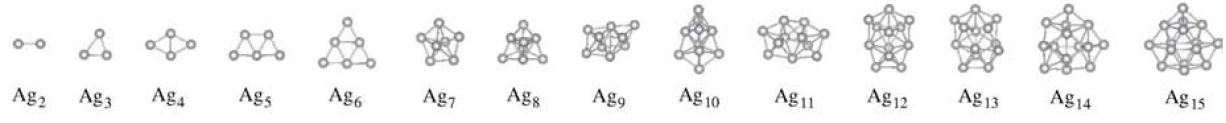
\includegraphics[width=1\textwidth]{images/estrutura_cluster_ag}
  \caption{ Exemplo de estruturas de \textit{Clusters} de prata.\cite{dissertacao_anderson}  }
  \label{fig:estrutura_cluster_ag}
\end{figure}


O histórico de estudo da organização espacial dos arranjos atômicos cristalinos frutificaram na premiação de um Nobel em 1915, para William Henry Bragg e William Lawrence Bragg, nota-se então a complexidade desse tipo de pesquisa. A análise das estruturas dos \textit{clusters} é fundamental para compreender suas propriedades e  dispor de seus potenciais tecnológicos, isso também torna-se muito importante para o domínio da estabilidade das nanopartículas. 

A análise da distribuição do tamanho dos \textit{clusters}, advindos dos espectros
de massa, pode prover critérios fundamentais para as tendências estruturais e energéticas \cite{dissertacao_anderson}, no qual está focado este trabalho.

Knight et al (68) encontraram picos bem definidos no espectro de massa de
clusters de Na em fase gasosa, especificamente, para clusters com 2, 18, 20, 34, 40, 58,...
átomos.(68) Esses picos referem-se à maior abundância e estabilidade desses tamanhos em
relação aos demais, os quais foram chamados clusters mágicos ou clusters com números
mágicos de átomos. A ocorrência desses clusters mágicos foi atribuída à efeitos de
preenchimento de camadas eletrônicas, em que a combinação entre o espectro de estados
quantizados e o princípio de exclusão de Pauli resulta em efeitos de camada, comum em
sistemas finitos de férmions como elétrons em átomos ou prótons e neutrons em núcleos
atômicos.(69) Posteriormente, os efeitos eletrônicos foram confirmados através de curvas
do potencial de ionização.(70) Esses mecanismos apresentam analogia com o modelo de
camadas em física nuclear(69) (similaridade que beneficia o estudo de clusters metálicos)
, principalmente clusters neutros em que forças eletrostáticas de longo alcance se anulam e
os elétrons de valência são ligados por interações de troca e correlação de curto alcance.



